\documentclass[13pt]{beamer}

\usetheme{Copenhagen}

\usecolortheme[rgb={0.60884,0.1590909,0.23106061}]{structure} % Red colors
\usefonttheme{serif}
\setbeamerfont{frametitle}{size=\normalsize}
 %\useoutertheme{mathRiponlogo}

%\setbeamertemplate{itemize/enumerate body begin}{\large}
%\setbeamertemplate{itemize/enumerate subbody begin}{\large}
\setbeamertemplate{navigation symbols}{}%remove navigation symbols

\usepackage[english]{babel}
\usepackage[utf8x]{inputenc}
\usepackage{multicol}
\usepackage{fmtcount}

\newcounter{count}
\addtocounter{count}{1}

\newcommand{\quotes}[2]{\centering \Large{``#1"\\
\vspace*{0.2in}
\hspace*{0.5in} - #2}}

\newcommand{\question}{ \textbf{(\decimal{count})} \stepcounter{count}}
\newcommand{\pic}[2]{\hfill\includegraphics[scale=#2]{#1}\hspace*{\fill}}

\newenvironment{stepenumerate}{\begin{enumerate}[<+->]}{\end{enumerate}}
\newenvironment{stepitemize}{\begin{itemize}[<+->]}{\end{itemize} }

\title{Section 1.1}
\author{Chester Ismay, Tom Linton}
\institute{Ripon College, Central College}
\date{}


\begin{document}

\begin{frame}
  \titlepage
\end{frame}

\begin{frame}{Learning Quote of the Day}
\quotes{It is not that I'm so smart. But I stay with the questions much longer.}{Albert Einstein}
\end{frame}

\begin{frame}{Recall from Exploration 1.1}

\question  What was the dog's name?
  \begin{enumerate}[A]
    \item Buzz
    \item Doris
    \item Harley%correct answer
    \item Sarah
    \item None of the above
  \end{enumerate}

\end{frame}

\begin{frame}{Explain the Results from Exploration 1.1}

Here are two possible explanations for why Harley chose the correct cup 9 out of 10 times:
\begin{itemize}
\item He was just guessing and got lucky in these 10 trials.
\item He is doing something other than merely guessing and perhaps understands what the
experimenter means when they bow towards the cup.
\end{itemize}

\question According to the simulated "chance model", which is the more plausible (more       likely to be correct) explanation?
  \begin{enumerate}[A]
    \item He is just guessing.
    \item There is something more than guessing happening here.%correct answer
    \item Both explanations are equally plausible.
    \item Neither explanation is plausible.
  \end{enumerate}

\end{frame}

\begin{frame}{Second Study}

\question After determining that 9 out of 10 correct cup choices with human gestures was     statistically significant, the researchers used a mechanical arm to point and Harley     got 6 out of 10 correct. Was this second result statistically significant?
  \begin{enumerate}[A]
    \item Yes, and I'm very confident.
    \item Yes, but I'm not sure.
    \item No, but I'm not sure.%Correct but unsure
    \item No, and I'm very confident.%Best answer
  \end{enumerate}

\end{frame}

\begin{frame}{Parameter in Exploration 1.1}
\question What is the parameter of interest in Exploration 1.1?
  \begin{enumerate}[A]
    \item The 10 trials
    \item The proportion of times Harley chooses the correct cup in 10 trials
    \item The long-run probability that Harley will choose the correct cup over many, many trials%Correct
    \item The number of times Harley chooses the correct cup
  \end{enumerate}

\end{frame}

\begin{frame}{Hypothesized value in Exploration 1.1}
\question Why do we select 0.50 as being the hypothesized value (\texttt{Probability of heads})?
  \begin{enumerate}[A]
    \item The chance model for One Proportion tests will be 0.50 regardless of the situation.
    \item This hypothesized value corresponds to the chance outcome of flipping a fair coin and getting a head.
    \item This is actually an error. We should have selected 0.90 since that is the proportion of the time Harley was correct.
    \item We could have picked any value between 0 and 1 and we just happened to pick 0.5.
  \end{enumerate}

\end{frame}

\begin{frame}{Section 1.1 Chance Models}
\begin{stepitemize}
  \item A result is \textbf{statistically significant} if it is unlikely to occur by chance alone. 
  \item We introduce \textit{chance models}, which help us determine if study results are statistically significant.
\end{stepitemize}
\end{frame}

\begin{frame}{Doris and Buzz}
\begin{center}
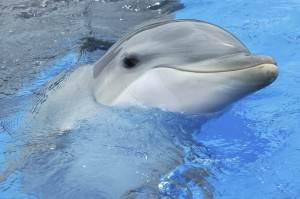
\includegraphics[width=2.37 in]{dolphin1.jpg}
\end{center}
\begin{stepitemize}
  \item Can dolphins communicate abstract ideas? 
  \item In an experiment done in the 1960s, Doris was instructed which of two buttons to push.  She then had to communicate this to Buzz (who could not see Doris).  If he picked the correct button, both dolphins would get a fish as a reward. 
\end{stepitemize}
\end{frame}

\begin{frame}{One trial}
\begin{stepitemize}
  \item Dr. Bastian would show the light (blinking or steady) to Doris. 
  \item Doris would swim over towards Buzz and the dolphins would exchange squeaks.
  \item Buzz would select one of the two buttons.
  \item If Buzz selected the correct button, both dolphins got a fish.
\end{stepitemize}
 \end{frame}

\begin{frame}{16 trials = 1 Repetition}
\question Dr. Bastian repeated this \textit{trial} 16 times and Buzz selected the correct button in 15 out of 16 trials. What are the observational units?
\begin{enumerate}[A]
  \item Buzz and Doris.%Decent answer
  \item Doctors.
  \item Dolphins.
  \item The trials.%Correct
  %\item The buttons.
\end{enumerate}
\end{frame}

\begin{frame}{Variable}
\question What is the variable of interest? \textbf{Hint:} the variable of interest must be a characteristic of the observational units.
\begin{enumerate}[A]
  \item The number of times Buzz pushed the correct button.
  \item The status of the light (steady or blinking).
  \item Whether or not Buzz pushed the correct button.%Correct
  \item If Doris and Buzz did better than guessing.
  \item The two different dolphins.
\end{enumerate}
\end{frame}

\begin{frame}{Are you convinced?}

\question  Doris and Buzz got 15 out of 16 button pushes correct, does this convince you that something more than just guessing is going on here?  Select the ``best'' response below.
%Any answer is fine here, the last 2 are desirable
  \begin{enumerate}[A]
    \item No,  15 out of 16 correct could easily be due to guessing.
    \item Not really, 15 out of 16 correct is a bit unusual, but I need more convincing.
    \item Maybe, maybe not, I am just not sure.
    \item Probably, guessing 15 out of 16 seems rare, but maybe they were super lucky.
    \item Yes, 15 out of 16 would almost never happen if they were just guessing.
  \end{enumerate}

\end{frame}

\begin{frame}{Justification and Model}
 \begin{stepitemize}
  \item How might we justify our answer to the last question? Discuss this with a small group of other students.
  %I would ask for solutions at this point
  
  \item Given a fair coin, how might we model the situation where Buzz is just guessing?
  \begin{stepenumerate}
    \item Heads = Buzz is correct, tails = incorrect
    \item Flip the coin 16 times and count the number of heads
    \item Repeat the last step many times to generate a distribution of what might happen if Buzz is just guessing.
    \item How does 15 out of 16 "fit" with  this "chance model"?
  \end{stepenumerate}
 % \item Take a coin and try it out.  %I am going to discuss 13a and 13b from the exploration at the beginning of class so I don't think we will need to have them flip again.
\end{stepitemize}
\end{frame}

\begin{frame}{The 3S Strategy}
\textbf{Statistic:} Compute a statistic from the study (15 out of 16 correct).\smallskip

\begin{multicols}{2}
\textbf{Simulate:} Identify a model that represents a chance explanation. Repeatedly simulate values of the statistic that could have happened when the chance model is true and form a distribution (coin flipping applet). 
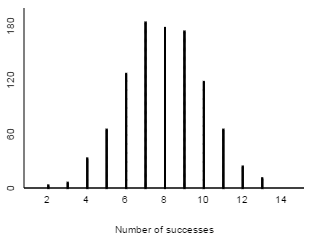
\includegraphics[width=2.37 in]{dolphindistribution.PNG}
\end{multicols}

\textbf{Strength of Evidence:} Consider whether the value of the observed statistic is unlikely to occur when the chance model is true (we never got 15 out of 16). 
\end{frame}

\begin{frame}{A Second Experiment}
\question With a wooden barrier replacing the canvas barrier, Buzz pushed the correct button 16 out of 28 times. Do you think this result is statistically significant?
%Any answer is fine here, the 1st 2 are desirable

\begin{enumerate}[A]
\item No
\item Probably not
\item I am unsure
\item Probably
\item Yes
\end{enumerate}
\end{frame}

\begin{frame}{A Second Experiment}
\question With a wooden barrier replacing the canvas barrier, Buzz pushed the correct button 16 out of 28 times. Use the one Proportion applet to decide if this result is statistically significant.
\begin{enumerate}[A]
\item No%Correct
\item Probably not%Ok answer
\item I am unsure
\item Probably
\item Yes
\end{enumerate}
\end{frame}

\begin{frame}{Summary}
This time, the study statistic, 16 out of 28 correct, happens 28 or 29\% of the time, when Buzz is just guessing, which is NOT statistically significant.
\begin{center}
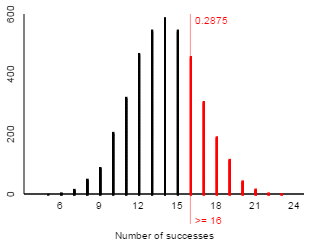
\includegraphics[width = 2.5 in]{dolphindistribution2.PNG}
\end{center}
\end{frame}
%--------------------------------------
\begin{frame}{Key Terms to Understand in Section 1.2}
\begin{multicols}{2}
\begin{itemize}
	\item Test of Significance
    \item Hypotheses
    \begin{itemize}
        \item Null Hypothesis, $H_0$
        \item Alternative Hypothesis, $H_a$
    \end{itemize}
    \item Parameter versus Statistic
    \item Binary Variable
    \item $p$-value
\end{itemize}
\end{multicols}
\end{frame}

\end{document}